\documentclass[12pt]{article}

\usepackage[english]{babel}
\usepackage[utf8]{inputenc}
\usepackage{sansmathfonts}
\usepackage[T1]{fontenc}
\renewcommand*\familydefault{\sfdefault} %% Only if the base font of the document is to be sans serif
\usepackage{multicol,lipsum}
\usepackage{amsmath,cancel}
\usepackage{amssymb,amsthm,dsfont,mathrsfs}
\usepackage[colorinlistoftodos]{todonotes}
\usepackage{geometry}
\geometry{
a4paper,
total={170mm,257mm},
left=20mm,
top=15mm,
bottom=22mm,
}
\usepackage{natbib}
\usepackage{soul}
\usepackage{setspace}
\usepackage{hyperref}
\usepackage{xcolor}
\usepackage{graphicx}
\usepackage{tikz}
\usepackage{siunitx}
\graphicspath{ {imagens/} }
\usepackage{fancyhdr}
\pagestyle{fancy}
\renewcommand{\headrulewidth}{0pt}

\color{darkgray}
\newcommand{\T}[1]{\vspace{0.4cm}\textbf{\large#1}}
\newcommand{\TW}[1]{\textbf{\large#1}}

\newcommand{\TM}[1]{\vspace{0.2cm} \textbf{#1}}

\newcommand{\M}[1]{
\vspace{-0.6cm}
\begin{flalign*}
#1&
\end{flalign*}
\vspace{-0.6cm}
}


\definecolor{bluebell}{rgb}{0.25, 0.35, 0.89} 
\definecolor{laranja}{rgb}{0.87, 0.48, 0.25} 
\definecolor{verde}{rgb}{0, 0.54, 0.44} 
\definecolor{babypink}{rgb}{1, 0.42, 0.52} 
\definecolor{rosa}{rgb}{1, 0.72, 0.77} 
\definecolor{cinza}{rgb}{0.3, 0.3, 0.3}  
\definecolor{iris}{rgb}{0.25, 0.35, 0.89}  
\definecolor{babyblue}{rgb}{0.13, 0.59, 0.95}

\setlength\columnsep{30pt}

\setlength{\parindent}{0cm}
\setlength{\fboxrule}{1.3pt}  % <-- Aumenta a espessura

\newcommand{\Formula}[1]{
\begin{center}
\color{iris}
\fcolorbox{rosa}{white}{
\(
\begin{array}{c}
#1
\end{array}
\)
}
\color{cinza}
\end{center}
}

\begin{document}
\pagenumbering{gobble}
\setstretch{1.3}


\includegraphics[width=4cm]{Logo2.png}
\begin{center}
    \textbf{\Huge \textcolor{bluebell}{Área e Perímetro}}
\end{center}

\begin{multicols}{2}

\TW{Definição}

A \textbf{área} de uma figura plana é a medida da superfície que ela ocupa — imagina-se a figura coberta por quadradinhos de lado 1: a quantidade de quadradinhos é a área. A unidade é sempre quadrática: cm², m², km², etc.

O \textbf{perímetro} de um polígono é a medida total do seu contorno, obtida pela soma de todos os seus lados. A unidade é linear: cm, m, km, etc.

\Formula{P = l_1 + l_2 + \cdots + l_n}

A seguir apresentamos as fórmulas para os principais polígonos.

\TM{Quadrado}

A área $A$ do quadrado pode ser calculada pela fórmula: 

\Formula{A = l^2}

Onde $l$ representa a medida do lado do quadrado.

\vspace{-0.4cm}
\begin{center}
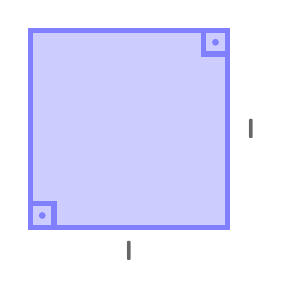
\begin{tikzpicture}
\tikzstyle{no}=[draw=none,fill=none,black!60!white]
\tikzstyle{line}=[blue!50!white,fill=blue!20!white,line width=2pt]
\draw[line] 
(0,0) rectangle (2.5,2.5);
\node[no] at (1.25,-0.3) {\textbf{l}};
\node[no] at (2.8,1.25) {\textbf{l}};
\draw[line] (0,0) rectangle (0.3,0.3);
\filldraw[blue!50!white] (0.15,0.15) circle (1pt);
\draw[line] (2.5,2.5) rectangle (2.2,2.2);
\filldraw[blue!50!white] (2.35,2.35) circle (1pt);
\end{tikzpicture}
\end{center}

Como o quadrado possui 4 lados com a mesma medida, então o perímetro $P$ pode ser calculado por:

\Formula{P = 4 \cdot l}

\TM{Exemplo:}

Se um quadrado tem lado $l=5$ então sua área $A = 25$. O mesmo pode ser feito para calcular a medida do lado do quadrado dada sua área. Por exemplo, se um quadrado possui área $A = 16$, então deduzimos que $l^2=16$, então $l= 4$.  

O perímetro de um quadrado com lado $l=3$ é $P=4 \cdot 3 = 12$.

\TM{Retângulo}

Dado um retângulo com base $b$ e altura $h$, temos que a área do retângulo é igual ao produto da medida da base pela altura. Ou seja:

\Formula{A = b \cdot h}

\vspace{-0.2cm}
\begin{center}
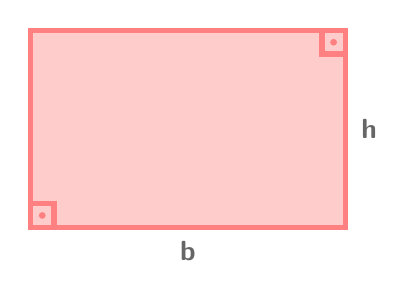
\begin{tikzpicture}
\tikzstyle{no}=[draw=none,fill=none,black!60!white]
\tikzstyle{line}=[red!50!white, fill=red!20!white, line width=2pt]
\draw[line] 
(0,0) rectangle (4,2.5);
\node[no] at (2,-0.3) {\textbf{b}};
\node[no] at (4.3,1.25) {\textbf{h}};
\draw[line] (0,0) rectangle (0.3,0.3);
\filldraw[red!50!white] (0.15,0.15) circle (1pt);
\draw[line] (4,2.5) rectangle (3.7,2.2);
\filldraw[red!50!white] (3.85,2.35) circle (1pt);
\end{tikzpicture}
\end{center}

Como o retângulo possui dois lados com a medida da base e dois lados com a medida da altura, então o perímetro pode ser calculado por:

\Formula{P = 2 \cdot (b+h)}

\TM{Exemplo:}

Dado um retângulo com base $b=4$ e altura $h=3$ temos:

$A = 4 \cdot 3 = 12$

O perímetro desse retângulo é calculado por:

$P = 2 \cdot (4+3) = 2 \cdot 7 = 14$

\TM{Paralelogramo}

A área do paralelogramo é idêntica a do retângulo, ou seja:

\Formula{A = b \cdot h}

\vspace{-0.4cm}
\begin{center}
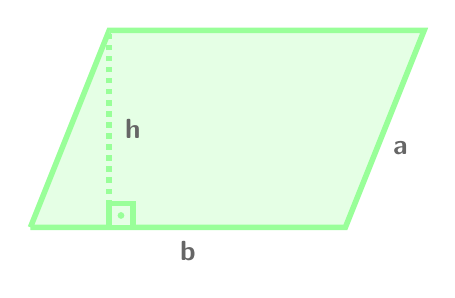
\begin{tikzpicture}
\tikzstyle{no}=[draw=none,fill=none,black!60!white]
\tikzstyle{line}=[green!40!white, fill=green!10!white, line width=2pt]
\draw[line] 
(0,0) -- (1,2.5) -- (5,2.5) -- (4,0) -- (0,0);
\node[no] at (2,-0.3) {\textbf{b}};
\node[no] at (4.7,1) {\textbf{a}};
\node[no] at (1.3,1.25) {\textbf{h}};
\draw[dotted,line] (1,0) -- (1,2.5);
\draw[line] (1,0) rectangle (1.3,0.3);
\filldraw[green!40!white] (1.15,0.15) circle (1pt);
\end{tikzpicture}
\end{center}

O perímetro do paralelogramo é semelhante ao perímetro do retângulo, a diferença é que no lugar a altura utiliza-se o lado $a$ do paralelogramo conforme a fórmula abaixo:

\Formula{P=2 \cdot (a+b)}

\TM{Exemplo:}

Dado um paralelogramo com base $b=5$, altura $h=2$ e lado $a=4$ temos:

$A = 5 \cdot 2 = 10$

$P = 2 \cdot (4+5) = 2 \cdot 9 = 18$

\TM{Triângulo}

A área do triângulo é calculada pela metade do produto da base $b$ pela altura $h$, deste modo temos:

\Formula{A = \dfrac{b \cdot h}{2}}

\vspace{-0.4cm}
\begin{center}
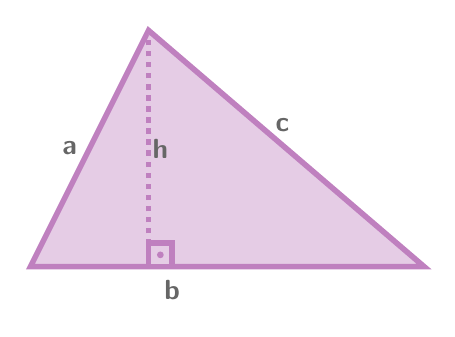
\begin{tikzpicture}
\tikzstyle{no}=[draw=none,fill=none,black!60!white]
\tikzstyle{line}=[violet!50!white, fill=violet!20!white, line width=2pt]
\draw[line] 
(0,0) -- (5,0) -- (1.5,3) -- cycle;
\draw[dotted,line] (1.5,0) -- (1.5,3);
\node[no] at (1.65,1.5) {\textbf{h}};
\node[no] at (0.5,1.5) {\textbf{a}};
\node[no] at (3.2,1.8) {\textbf{c}};
\node[no] at (1.8,-0.3) {\textbf{b}};
\draw[line] (1.5,0) rectangle (1.8,0.3);
\filldraw[violet!50!white] (1.65,0.15) circle (1pt);
\end{tikzpicture}
\end{center}

O perímetro do triângulo é calculado pela soma dos seus lados da seguinte forma:

\Formula{P=a + b + c}

\TM{Exemplo:}

Dado um triângulo com base $b=6$ e altura $h=3$ temos:

\vspace{8pt}
$A = \dfrac{6 \cdot 3}{2} = \dfrac{18}{2} = 9$ 
\vspace{8pt}

O perímetro de um triângulo com lados $a=3$, $b=6$ e $c=5$ é:

$P=3+6+5=14$

\TM{Triângulo Equilátero}

O triângulo equilátero é aquele que possui os três lados com a mesma medida. O cálculo da sua área é expresso pela fórmula:

\Formula{A = \dfrac{l^2 \sqrt{3}}{4}}

\vspace{-0.4cm}
\begin{center}
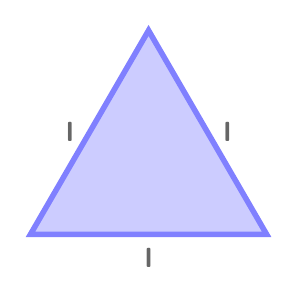
\begin{tikzpicture}
\tikzstyle{no}=[draw=none,fill=none,black!60!white]
\tikzstyle{line}=[blue!50!white,fill=blue!20!white,line width=2pt]
\draw[line] 
(0,0) -- (3,0) -- (1.5,2.59) -- cycle;
\node[no] at (1.5,-0.3) {\textbf{l}};
\node[no] at (0.5,1.3) {\textbf{l}};
\node[no] at (2.5,1.3) {\textbf{l}};
\end{tikzpicture}
\end{center}

Como o triângulo equilátero possui os três lados com a mesma medida o cálculo do seu perímetro é:

\Formula{P = 3 \cdot l}

\TM{Exemplo:}

Dado um triângulo equilátero com lado $l=4$ temos:

\vspace{8pt}
$A = \dfrac{4^2 \cdot \sqrt{3}}{4} = \dfrac{16 \cdot \sqrt{3}}{4} = 4 \sqrt{3}$ 
\vspace{8pt}

O perímetro desse mesmo triângulo é:

$P=3 \cdot 4=12$

\TM{Trapézio}

A área do trapézio é dada pela metade do produto da soma das bases pela altura. Em outras palavras temos que a área de um trapézio de base maior $B$, base menor $b$ e altura $h$ é a formula:  

\Formula{A = \dfrac{(B + b) \cdot h}{2}}

\vspace{-0.4cm}
\begin{center}
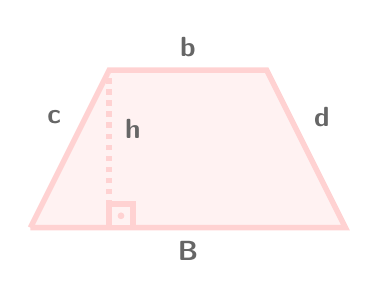
\begin{tikzpicture}
\tikzstyle{no}=[draw=none,fill=none,black!60!white]
\tikzstyle{line}=[pink!70!white, fill=pink!20!white, line width=2pt]
\draw[line] 
(0,0) -- (1,2) -- (3,2) -- (4,0) -- (0,0);
\node[no] at (2,-0.3) {\textbf{B}};
\node[no] at (1.3,1.25) {\textbf{h}};
\node[no] at (2,2.3) {\textbf{b}};
\node[no] at (0.3,1.4) {\textbf{c}};
\node[no] at (3.7,1.4) {\textbf{d}};
\draw[dotted,line] (1,0) -- (1,2);
\draw[line] (1,0) rectangle (1.3,0.3);
\filldraw[pink!70!white] (1.15,0.15) circle (1pt);
\end{tikzpicture}
\end{center}

O perímetro do trapézio é dado pela soma dos seus quatro lados:

\Formula{P=B+b+c+d}

\TM{Exemplo:}

Dado um trapézio com base maior $B=7$, base menor $b=3$, altura $h=2$ e lados $c=d=4$ temos:

\vspace{8pt}
$A = \dfrac{(7 + 3) \cdot 2}{2} = 10$
\vspace{8pt}

$P=7+3+4+4=18$

\TM{Losango}

A área do losango é igual a metade do produto da diagonal maior $D$ pela diagonal menor $d$. 

\Formula{A = \dfrac{D \cdot d }{2}}

\vspace{-0.4cm}
\begin{center}
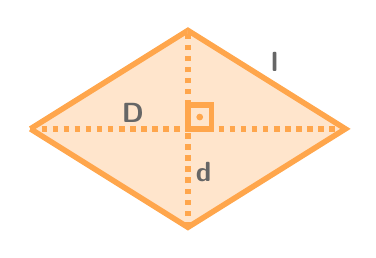
\begin{tikzpicture}
\tikzstyle{no}=[draw=none,fill=none,black!60!white]
\tikzstyle{line}=[orange!70!white, fill=orange!20!white, line width=2pt]
\draw[line] 
(0,1.25) -- (2,2.5) -- (4,1.25) -- (2,0) -- (0,1.25);
\node[no] at (2.2,0.7) {\textbf{d}};
\node[no] at (1.3,1.45) {\textbf{D}};
\node[no] at (3.1,2.1) {\textbf{l}};
\draw[dotted,line] (2,0) -- (2,2.5);
\draw[dotted,line] (0,1.25) -- (4,1.25);
\draw[line] (2,1.25) rectangle (2.3,1.55);
\filldraw[orange!70!white] (2.15,1.4) circle (1pt);
\end{tikzpicture}
\end{center}

Como o losango possui 4 lados com a mesma medida, então o perímetro pode ser calculado por:

\Formula{P=4 \cdot l}

As diagonais do losango são perpendiculares e se bissectam, formando quatro triângulos retângulos com catetos $D/2$ e $d/2$ e hipotenusa $l$. Pelo Teorema de Pitágoras:

\Formula{l = \sqrt{\left(\dfrac{D}{2}\right)^2 + \left(\dfrac{d}{2}\right)^2}}

\TM{Exemplo:}

Dado um losango com diagonal maior $D=8$ e diagonal menor $d=6$ temos:

$l = \sqrt{4^2 + 3^2} = \sqrt{16+9} = \sqrt{25} = 5$

$A = \dfrac{8 \cdot 6}{2} = 24$ \qquad $P = 4 \cdot 5 = 20$

\TM{Círculo}

A área do círculo é calculada por meio do seu raio $r$ da seguinte forma: 

\Formula{A= \pi r^2}

\vspace{-0.5cm}
\begin{center}
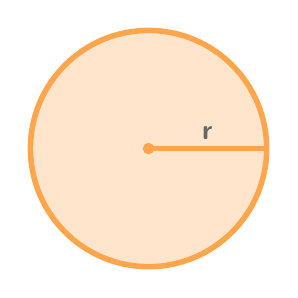
\begin{tikzpicture}
\tikzstyle{no}=[draw=none,fill=none,black!60!white]
\tikzstyle{line}=[orange!70!white, fill=orange!20!white, line width=2pt]
\draw[line] (0,0) circle (1.5);
\filldraw [line] (0,0) circle (1pt);
\draw[line] (0,0) -- (1.5,0);
\node[no] at (0.75,0.2) {\textbf{r}};
\end{tikzpicture}
\end{center}

O comprimento da circunferência é dado por:

\Formula{C= 2 \cdot \pi r}

\TM{Exemplo:}

Dado um círculo de raio $r=3$ temos:

$A = \pi \cdot 3^2 = 9\pi$

$C = 2\pi \cdot 3 = 6\pi$

\end{multicols}

\lfoot{\scriptsize © Copyright, Pratique Já}
\cfoot{\large \textcolor{bluebell}{pratiqueja.com}}
\end{document}